\documentclass{article}
\usepackage{graphicx}
\usepackage{tikz}
\usepackage{amsmath}
\usepackage{float}
\usepackage[margin=1in]{geometry}
\usetikzlibrary{positioning,fit,calc,arrows}

\usepackage{fancyhdr}
\pagestyle{fancyplain}
\fancyhf{}
\fancyhead[C]
{
    Feuchtraumabzweigdose PCB\hfill
    \thepage \\
    Prototyping Playground for the Open Bike Project\hfill
    spacecarrot, Feb 2020}
\renewcommand{\headrulewidth}{1.5pt}


\begin{document}
\noindent
\section{Power Section}
The board can be directly supplied from any 3.3Vdc/500mA source. There's also some optional sections to efficiently interface with a protected single cell Li+ battery and most bicycle dynamos. Here's a flowchart:

\begin{figure}[h]
    \centering
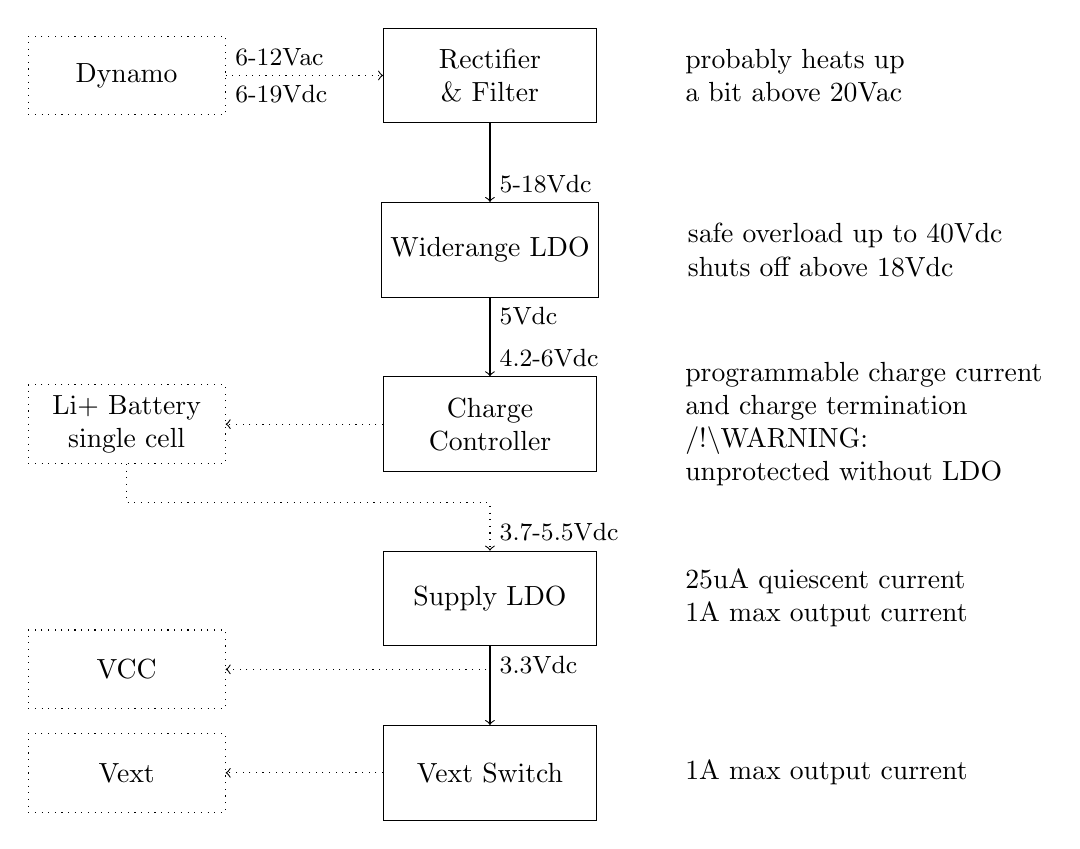
\begin{tikzpicture}
    \draw
        node[align=center,draw,minimum width=2.7cm,minimum height=1.2cm] (rect) {Rectifier\\ \& Filter}

        node[align=center,draw,below=of rect,minimum width=2.7cm,minimum height=1.2cm] (ldo) {Widerange LDO}
        node[align=center,draw,below=of ldo,minimum width=2.7cm,minimum height=1.2cm] (charge) {Charge\\Controller}
        node[align=center,draw,below=of charge,minimum width=2.7cm,minimum height=1.2cm] (supply) {Supply LDO}
        node[align=center,draw,below=of supply,minimum width=2.7cm,minimum height=1.2cm] (switch) {Vext Switch}

        node[dotted,align=center,draw,left=2cm of rect,minimum width=2.5cm,minimum height=1cm] (dyn) {Dynamo}
        node[dotted,align=center,draw,left=2cm of charge,minimum width=2.5cm,minimum height=1cm] (batt) {Li+ Battery\\single cell}
        node[dotted,align=center,draw,left=2cm of switch,minimum width=2.5cm,minimum height=1cm] (vext) {Vext}
        node[dotted,align=center,draw,above=0.3cm of vext,minimum width=2.5cm,minimum height=1cm] (vcc) {VCC}

        node[align=left,right=1cm of rect] {probably heats up\\a bit above 20Vac}
        node[align=left,right=1cm of supply] {25uA quiescent current\\1A max output current}
        node[align=left,right=1cm of ldo] {safe overload up to 40Vdc\\shuts off above 18Vdc}
        node[align=left,right=1cm of charge] {programmable charge current\\and charge termination\\/!\textbackslash WARNING:\\unprotected without LDO}
        node[align=left,right=1cm of switch] {1A max output current}

        node[right=0cm of dyn,align=left,anchor=south west] {\small 6-12Vac}
        node[right=0cm of dyn,align=left,anchor=north west] {\small 6-19Vdc}
        node[above=0cm of ldo,anchor=south west] {\small 5-18Vdc}
        node[below=0cm of ldo,anchor=north west] {\small 5Vdc}

        node[above=0cm of charge,anchor=south west] {\small 4.2-6Vdc}
        node[above=0cm of supply,anchor=south west] {\small 3.7-5.5Vdc}
        node[below=0cm of supply,anchor=north west] {\small 3.3Vdc}
    ;
    \draw [->] (rect)-- (ldo);
    \draw [->] (ldo)-- (charge);
    \draw [->] (supply)-- (switch);

    \draw[->,dotted] (dyn)-- (rect);
    \draw[->,dotted] (charge)-- (batt);
    \draw[->,dotted] (supply)|- (vcc);
    \draw[->,dotted] (switch)-- (vext);
    \draw[->,dotted] (batt)|- ++(0,-1)-| (supply);
\end{tikzpicture}
    \caption{Dependency Flowchart}
\end{figure}

\subsection{Rectifier \& Filter}
Due to space limitations, there is no filter coil, but the inductance of the dynamo itself should suffice to provide reasonably low ripple at average driving speed. By adjusting the charge current of the charge controller ripple can be further reduced if necessary. A 22V Zener clamps with a reasonable safety ratio to the 35V electrolyte. The rectifier pads can be soldered together pairwise to allow for 5-18Vdc at the Dynamo header if ac is not needed, with the header row labelled '1' serving as positive supply and '2' as ground.
\begin{figure}[h]
\centering
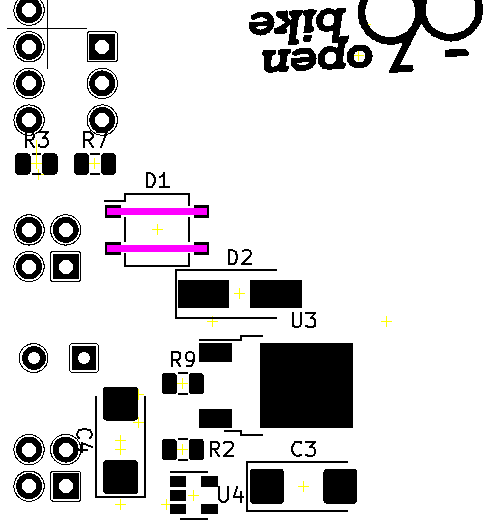
\includegraphics[height=4cm] {bridge.png}
\caption{Bridged Rectifier}
\end{figure}
\\BOM: D1, D2, C2, Charge Controller and Widerange LDO section

\subsection{Widerange LDO}
When overvolted, the charge controller would probably in return overvolt the battery, which is generally considered a messy thing. The widerange LDO can deal with inputs up to 40Vdc, although it shuts down at 18Vdc. Max current 500mA, supply current 500uA, 0.45V dropout. It's prudent to use the input stabilization and protection even when the board is configured for dc only.
\newline \newline
BOM: U3, D2, C2, Charge Controller section

\subsection{Charge Controller}
The charge controller takes anything between Vbatt+0.3V to 6V and charges a single cell Li+ battery in constant current mode for Vbatt<4.2V, then switches to constant voltage mode and finally terminates the charge when the charge current drops to prolong the lifetime of the battery.\\
The charge current during the constant current phase, the preconditioning current and the charge termination current can be programmed in tandem with R2:

\begin{align*}
I_{charge} &\propto R_2^{-1}\\
I_{charge}^{max}/R_2^{min}&=500mA/2k\\\\\\
I_{charge}^{stock}/R_2^{stock}&=100mA/10k\\
I_{termination}/I_{charge}&=0.05\\
I_{preconditioning}/I_{charge}&=0.1
\end{align*} 
/!\textbackslash WARNING: If a voltage above 6V is applied the internal controller is somewhat undefined and might let more through then you might want on a Li+, so be really sure your source is safe. If you want additional protection, look into the next section.
\newline \newline
BOM: C4,R2,C3,U4

\subsection{Supply LDO}
The digital section has a single 3.3Vdc power supply. If 3.3V are externally supplied via the VCC header, R3, R7 and U5 should be omitted. The input of the LDO should never be below the output by more than 0.3V or damage to the regulator can occur.
\newline \newline
/!\textbackslash WARNING: Do not connect an external supply while a battery is connected. Unregulated reverse current into a Li+battery is bad. Also note that there is no undervoltage protection for the battery, so do not use unprotected batteries. 
\begin{figure}[h]
\centering
\begin{tabular}{ l l }
    Module & Quiescent Current \\
    \hline
    Supply LDO & 25uA  \\
    Voltage Dividers + Comparator & 1uA \\
    Vext Switch & 1uA \\
    ESP32 (Deep Sleep) & 5uA \\
    MPU9250 (Sleep) & 8uA \\
    RFM95W (Deep Sleep) & 1uA \\
    \hline
    total & 41uA \\
\end{tabular}
\caption{Sleep Depth}
\end{figure}
\\BOM: C4, U5

\subsection{Vext Switch}
This can be used to switch off power hungry external modules during sleep. If the inrush current is too high for the supply to handle, adding a small (\textasciitilde 1-10nF) capacitor as C1 may help against ESP32 brownouts.
\newline \newline
BOM: R1, R5, C1, Q1
\section{Interfaces}

\begin{figure}[H]
    \centering
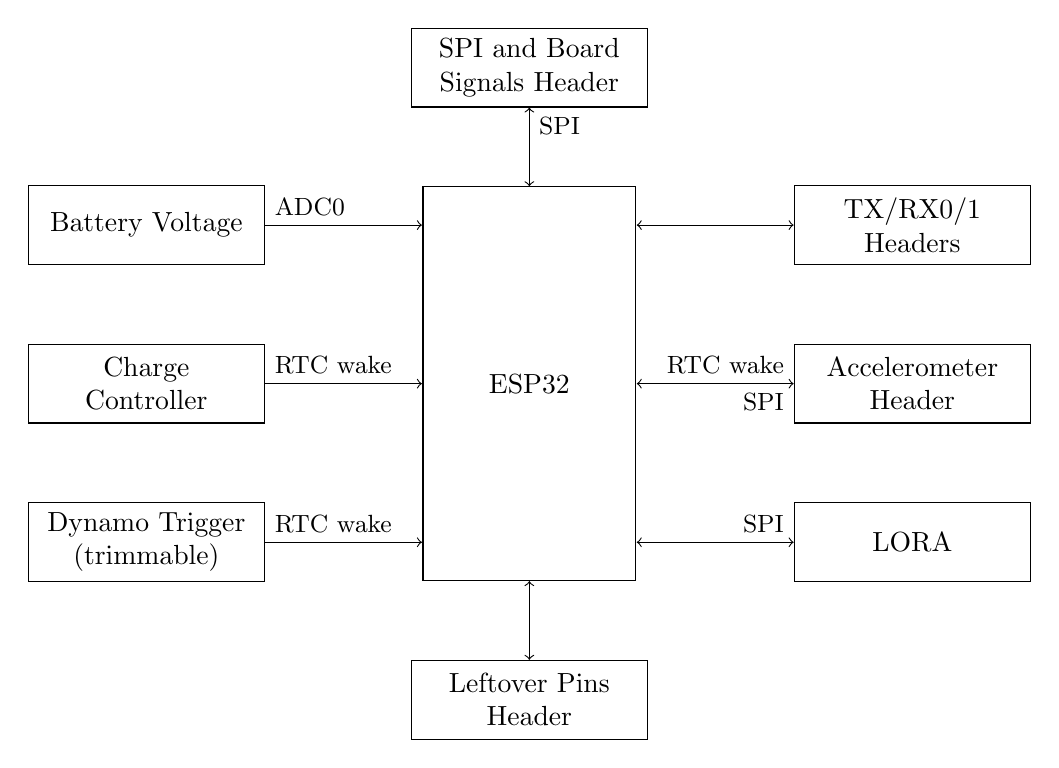
\begin{tikzpicture}
    \draw
        node[align=center,draw,minimum width=2.7cm,minimum height=5cm] (esp) {ESP32}
        
        node[align=center,draw,below=of esp,minimum width=3cm, minimum height=1cm] (misc) {Leftover Pins\\Header}
        node[align=center,draw,above=of esp,minimum width=3cm,minimum height=1cm] (spi) {SPI and Board\\Signals Header}
        node[below=0cm of spi,align=left,anchor=north west] {\small SPI}

        node[align=center,draw,left=2cm of esp,minimum width=3cm,minimum height=1cm] (charge) {Charge\\Controller}
        node[right=0cm of charge,align=left,anchor=south west] {\small RTC wake}

        node[align=center,draw,above=of charge,minimum width=3cm,minimum height=1cm] (batt) {Battery Voltage}
        node[right=0cm of batt,align=left,anchor=south west] {\small ADC0}


        node[align=center,draw,below=of charge,minimum width=3cm,minimum height=1cm] (dynamo) {Dynamo Trigger\\(trimmable)}
        node[right=0cm of dynamo,align=left,anchor=south west] {\small RTC wake}

        node[align=center,draw,right=2cm of esp,minimum width=3cm,minimum height=1cm] (mpu) {Accelerometer\\Header}
        node[left=0cm of mpu,align=left,anchor=south east] {\small RTC wake}
        node[left=0cm of mpu,align=left,anchor=north east] {\small SPI}

        node[align=center,draw,above=of mpu,minimum width=3cm,minimum height=1cm] (serial) {TX/RX0/1\\Headers}

        node[align=center,draw,below=of mpu,minimum width=3cm,minimum height=1cm] (lora) {LORA}
        node[left=0cm of lora,align=left,anchor=south east] {\small SPI}

    ;

    \draw[<->] (misc)-- (esp);
    \draw[<->] (spi)-- (esp); 
    \draw[->] (batt)-- ++(3.5cm,0);
    \draw[->] (charge)-- ++(3.5cm,0);
    \draw[->] (dynamo)-- ++(3.5cm,0);
    \draw[<->] (serial)-- ++(-3.5cm,0);
    \draw[<->] (mpu)-- ++(-3.5cm,0);
    \draw[<->] (lora)-- ++(-3.5cm,0);
\end{tikzpicture}
    \caption{Interfaces}
\end{figure}

\subsection{Battery Voltage}
The battery voltage can be read via a voltage divider on the ADC0 bank. The 1/10 voltage divider sacrifices resolution for reduced current draw. Note that the ESP32 ADCs are not very linear, and also that the ADC1 bank does not work if wifi is enabled.
\newline \newline
BOM: R3, R7, Supply LDO section
\subsection{Charge and Dynamo Wakeup}
The charge controller can send its charge state to the ESP32 with a single resistor. Additionally, a trimmable comparator can detect lower voltages at the input of the wide range LDO and send a wakeup signal on slight movement. The trim range by default is 0-7.35V, when a lower range is desired for better adjustment R6 can be increased to 470k for a range of 0-1V.
\newline \newline
BOM Charge: R9, Charge Controller section\\
BOM Dynamo: R8, R6 ,R10, R11, RV1, D3, U6, Charge Controller and Widerange LDO section
\subsection{Accelerometer Header}
There's a common cheap prototyping board for the MPU 9250 that can be directly installed here.
\subsection{Leftover Pins Header}
This header exposes all the unused pins. Please note that some of them have special properties such as blocking the boot process or accessing the onboard flash. Consult the datasheet or look online for explanations if undesired side effects occur.
\subsection{SPI and Board Signals Header}
The system is designed for a common SPI bus. This is generally not problematic, but different devices may use different configurations in terms of clock idle state etc.; switching these protocols depending on the selected slave may be necessary in software.\\
The board signals are also exposed. Note that interfering with them might interfere with them, however if a section is not installed those can be used as additional GPIOs.

\section*{Annex}
\subsection*{Pin Configuration}
\begin{figure}[h]
\centering
\begin{tabular}{ l l }
    GPIO & Function \\
    \hline
    1 & TX0\\
    2 & $\overline{\textrm{Charge}}$ (configure as pullup)\\
    3 & RX0\\
    4 & MPU9250 Wake \\
    5 & MPU9250 SPI Select \\
    15 & Dynamo Wake\\
    16 & RX1 \\
    17 & TX1 \\
    18 & SPI Clock \\
    19 & SPI MISO \\
    21 & RFM95W SPI Select\\
    23 & SPI MOSI \\
    26 & RFM95W Digital IO0\\
    27 & RFM95W Digital IO1\\
    32 & Battery ADC\\
    33 & RFM95W Reset
\end{tabular}
\end{figure}

\subsection*{List of optional components}
\begin{figure}[h]
\centering
\begin{tabular}{l}
    R1, R2, R3, R5, R6, R7, R8, R9, R10, R11, RV1\\
    C1, C2, C3, C4\\
    D1, D2, D3, Q1, U3, U4, U5, U6
\end{tabular}
\end{figure}
\end{document}

